\documentclass[tikz,border=8pt]{standalone}
\usepackage[T1]{fontenc}
\usepackage[utf8]{inputenc}
\usetikzlibrary{positioning,arrows.meta}
\begin{document}
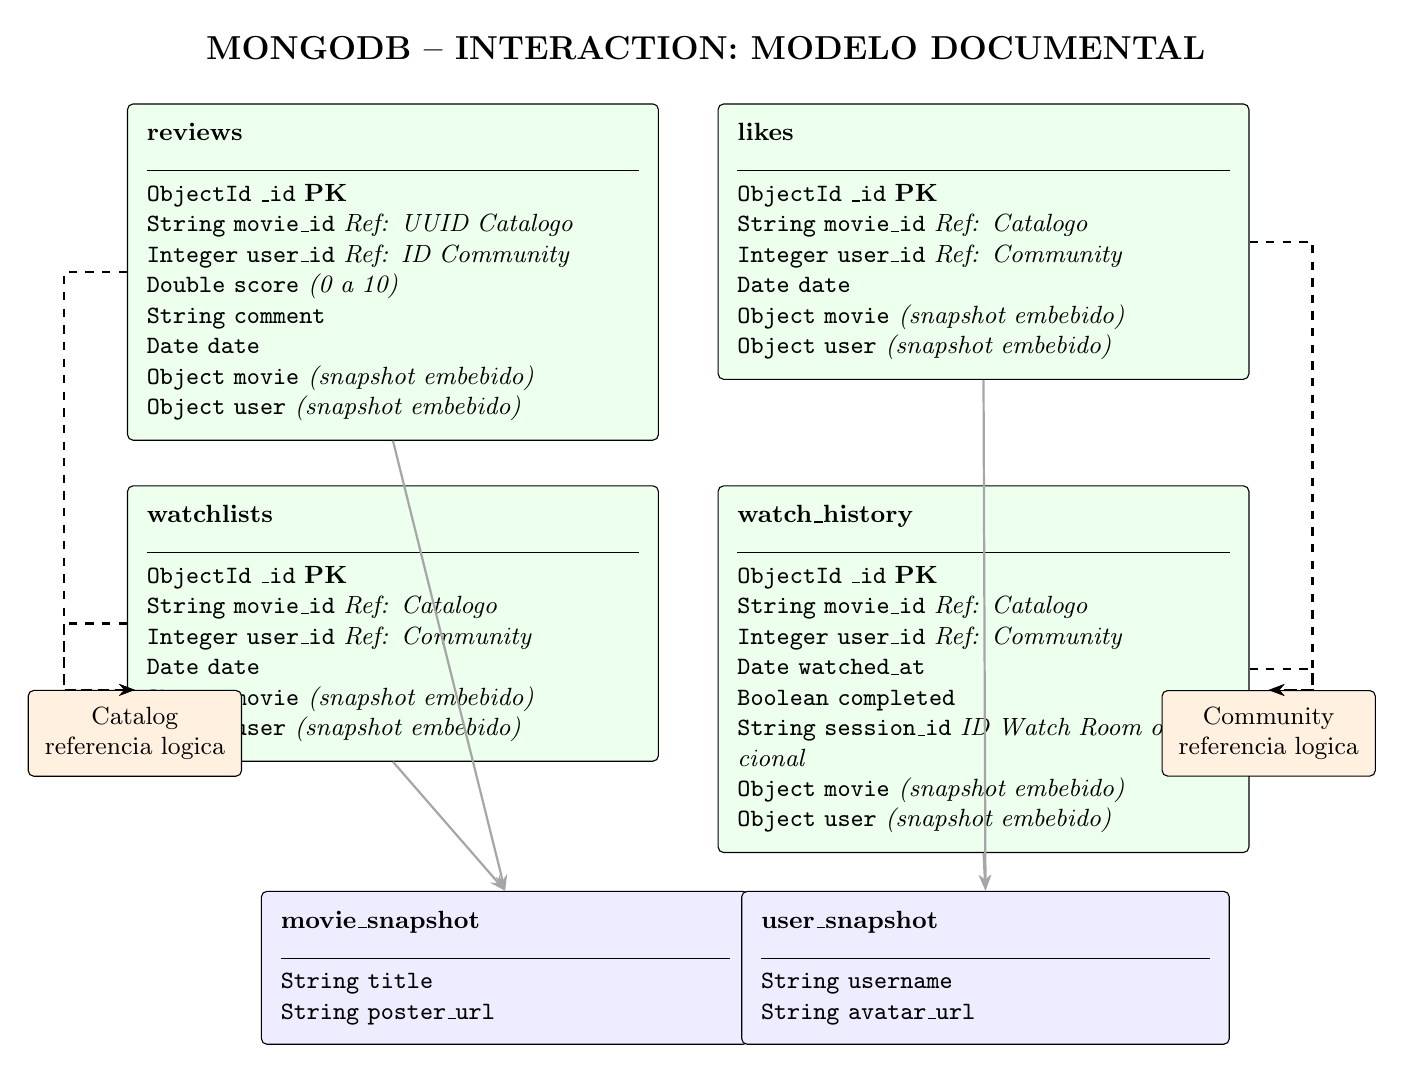
\begin{tikzpicture}[
  font=\small,
  collection/.style={draw, rounded corners=2pt, align=left, text width=6.25cm,
    inner sep=7pt, fill=green!7},
  snapshot/.style={draw, rounded corners=2pt, align=left, text width=5.7cm,
    inner sep=7pt, fill=blue!7},
  external/.style={draw, rounded corners=2pt, align=center, inner sep=6pt,
    fill=orange!12},
  logical/.style={-{Stealth[length=2mm]}, dashed, thick},
  embedded/.style={-{Stealth[length=2mm]}, thick, gray!70},
  heading/.style={font=\bfseries\large}
]
\node[heading] (title) at (0,8.45) {MONGODB -- INTERACTION: MODELO DOCUMENTAL};

\node[collection, anchor=north west] (reviews) at (-7.35,7.75) {\textbf{reviews}\\\rule{6.25cm}{0.3pt}
\texttt{ObjectId \_id} \textbf{PK}\\
\texttt{String movie\_id} \textit{Ref: UUID Catalogo}\\
\texttt{Integer user\_id} \textit{Ref: ID Community}\\
\texttt{Double score} \textit{(0 a 10)}\\
\texttt{String comment}\\
\texttt{Date date}\\
\texttt{Object movie} \textit{(snapshot embebido)}\\
\texttt{Object user} \textit{(snapshot embebido)}};

\node[collection, anchor=north west] (likes) at (0.15,7.75) {\textbf{likes}\\\rule{6.25cm}{0.3pt}
\texttt{ObjectId \_id} \textbf{PK}\\
\texttt{String movie\_id} \textit{Ref: Catalogo}\\
\texttt{Integer user\_id} \textit{Ref: Community}\\
\texttt{Date date}\\
\texttt{Object movie} \textit{(snapshot embebido)}\\
\texttt{Object user} \textit{(snapshot embebido)}};

\node[collection, anchor=north west] (watchlists) at (-7.35,2.9) {\textbf{watchlists}\\\rule{6.25cm}{0.3pt}
\texttt{ObjectId \_id} \textbf{PK}\\
\texttt{String movie\_id} \textit{Ref: Catalogo}\\
\texttt{Integer user\_id} \textit{Ref: Community}\\
\texttt{Date date}\\
\texttt{Object movie} \textit{(snapshot embebido)}\\
\texttt{Object user} \textit{(snapshot embebido)}};

\node[collection, anchor=north west] (history) at (0.15,2.9) {\textbf{watch\_history}\\\rule{6.25cm}{0.3pt}
\texttt{ObjectId \_id} \textbf{PK}\\
\texttt{String movie\_id} \textit{Ref: Catalogo}\\
\texttt{Integer user\_id} \textit{Ref: Community}\\
\texttt{Date watched\_at}\\
\texttt{Boolean completed}\\
\texttt{String session\_id} \textit{ID Watch Room opcional}\\
\texttt{Object movie} \textit{(snapshot embebido)}\\
\texttt{Object user} \textit{(snapshot embebido)}};

\node[snapshot, anchor=north west] (movie) at (-5.65,-2.25) {\textbf{movie\_snapshot}\\\rule{5.7cm}{0.3pt}
\texttt{String title}\\
\texttt{String poster\_url}};
\node[snapshot, anchor=north west] (user) at (0.45,-2.25) {\textbf{user\_snapshot}\\\rule{5.7cm}{0.3pt}
\texttt{String username}\\
\texttt{String avatar\_url}};

\node[external] (catalog) at (-7.25,-0.25) {Catalog\\referencia logica};
\node[external] (community) at (7.15,-0.25) {Community\\referencia logica};

\draw[logical] (reviews.west) -- ++(-0.8,0) |- (catalog.north);
\draw[logical] (watchlists.west) -- ++(-0.8,0) |- (catalog.north);
\draw[logical] (likes.east) -- ++(0.8,0) |- (community.north);
\draw[logical] (history.east) -- ++(0.8,0) |- (community.north);
\draw[embedded] (reviews.south) -- (movie.north);
\draw[embedded] (likes.south) -- (user.north);
\draw[embedded] (watchlists.south) -- (movie.north);
\draw[embedded] (history.south) -- (user.north);

\end{tikzpicture}
\end{document}
